%------------------------------------------------
%----------------------------------------------------------------------------------------
\section{DWARF}
%----------------------------------------------------------------------------------------
%------------------------------------------------

\begin{frame}{DWARF}
    \begin{itemize}
	    \item Debugging with Attributed Record Formats(DWARF)
	    \item Debug information format
	    \item Rust uses DWARF version 4
	    \item DWARF is devided into 12 sections
	    \item Executable and Linkable Format(ELF)
    \end{itemize}
\end{frame}

%------------------------------------------------
%------------------------------------------------

\begin{frame}{DWARF Sections}
	\begin{figure}
		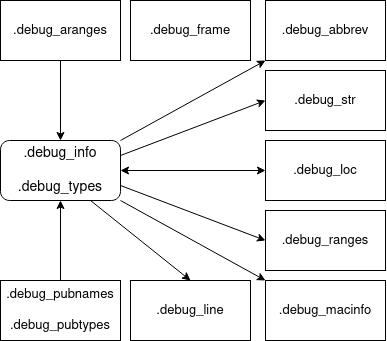
\includegraphics[width=0.9\textwidth,height=0.48\textwidth,keepaspectratio]{dwarf-sections.png}
	\end{figure}
\end{frame}

%------------------------------------------------
%------------------------------------------------

\begin{frame}{Debug Information Entry(DIE)}
	\begin{itemize}
	    \item DebugInformation Entry(DIE).
	    \item DWARF Attributes.
	    \item DWARF DIE example from the .debug\_info section.
	\end{itemize}
	\begin{figure}
		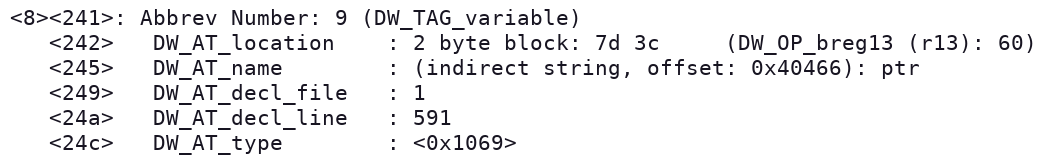
\includegraphics[width=0.9\textwidth,height=0.48\textwidth,keepaspectratio]{dwarf-die.png}
	\end{figure}
\end{frame}

%------------------------------------------------
%------------------------------------------------

\begin{frame}{Compilation unit}
	\begin{itemize}
		\item Computer program is devieded into compilation units.
		\item Each compilation unit contains a DIE tree.
	\end{itemize}
\end{frame}

%------------------------------------------------
%------------------------------------------------

\begin{frame}{Compilation unit}
	\begin{figure}
		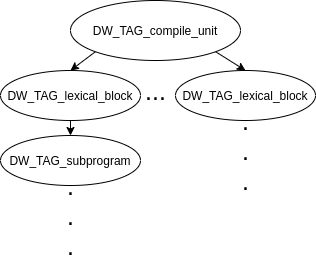
\includegraphics[width=0.9\textwidth,height=0.48\textwidth,keepaspectratio]{die-tree.png}
	\end{figure}
\end{frame}

%------------------------------------------------
%------------------------------------------------

\begin{frame}{Evaluating a variable}
	\begin{itemize}
		\item Find the current compilation unit.
		\item Find the current subprogram die.
		\item Find the searched variable die. 
		\item Two parts to evaluating a variable:
			\begin{itemize}
				\item Finding the location of the variable
				\item Parsing the value into the correct type
			\end{itemize}
	\end{itemize}
\end{frame}

%------------------------------------------------
%------------------------------------------------

\begin{frame}{Evaluating the location of a variable}
	\begin{figure}
		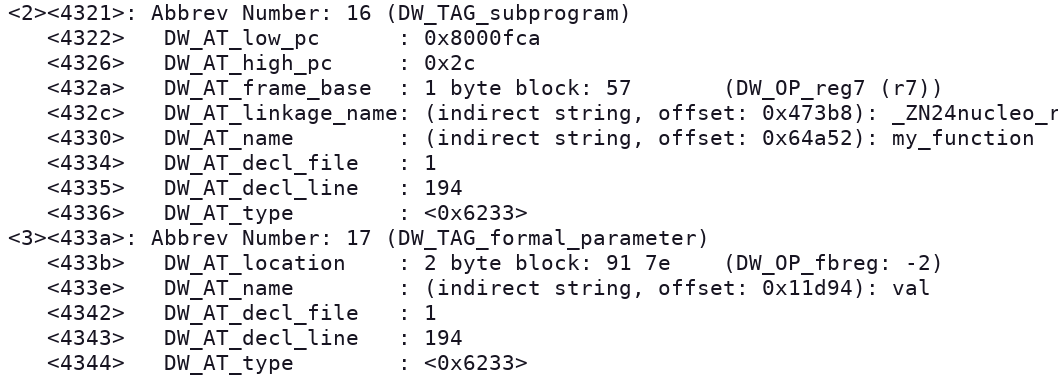
\includegraphics[width=0.9\textwidth,height=0.48\textwidth,keepaspectratio]{subprogram-example.png}
	\end{figure}
\end{frame}

%------------------------------------------------
%------------------------------------------------

\begin{frame}{Parsing the type of a variable}
	\begin{figure}
		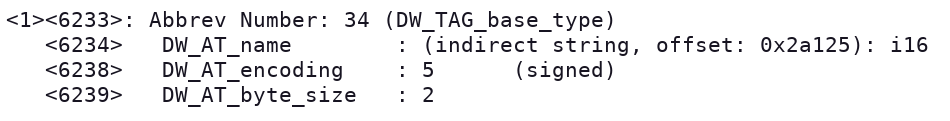
\includegraphics[width=0.9\textwidth,height=0.48\textwidth,keepaspectratio]{basetype-example.png}
	\end{figure}
\end{frame}

%------------------------------------------------
%------------------------------------------------

\begin{frame}{Virtually Unwinding Call Stack}
    \begin{itemize}
        \item Stack of subroutine activations.
        \item A subroutine activation consists of:
    	\begin{itemize}
    	    \item Code location were the subroutine stopped
    	    \item Preserved register values
	    \item Canonical Frame Address (CFA)
    	\end{itemize}
        \item The needed infomarion is in section .debug\_frame
    \end{itemize}
\end{frame}

%------------------------------------------------
%------------------------------------------------

\begin{frame}{Virtually Unwinding Subroutine Activations}
    \begin{columns}[c] % The "c" option specifies centered vertical alignment while the "t" option is used for top vertical alignment

        \column{.45\textwidth} % Left column and width
        \begin{enumerate}
        	\item Find the Common Information Entry (CIE)
		\item Find the Frame Description Entry (FDE)
		\item Unwind CFA and register values.
		\item Repeat for all activations.
        \end{enumerate}

        \column{.5\textwidth} % Right column and width
	\begin{figure}
		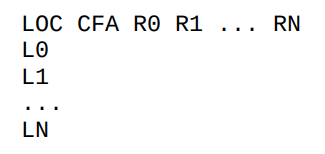
\includegraphics[width=0.9\textwidth,height=0.48\textwidth,keepaspectratio]{stacktrace-table.png}
	\end{figure}
    \end{columns}

\end{frame}

%------------------------------------------------

